\newpage

\setcounter{page}{1}
\setcounter{figure}{0}
\section{Uvod}% (fold)
\label{sec:Uvod}

\subsection{Zadatak diplomskog rada} % (fold)
\label{sub:Zadatak diplomskog rada}
\textbf{PRIVREMEN C/P opisa diplomskog} 
\\
Program RGBDSLAM raspoloživ u okviru programske biblioteke OpenSLAM
omogućava izgradnju 3D modela objekata i scena pomoću 3D kamere.
Razviti program za izgradnju 3D modela u obliku mreže trokuta koristeći
biblioteku PointCloud. Kombinacijom ova dva programa mogu se izgraditi
3D modeli objekata i scena snimljenih iz više pogleda. Zadatak je
ispitati funkcionalnost navedenog postupka kao i kvalitetu dobivenog
rezultata izgradnjom nekoliko 3D modela objekata i scena.

\begin{figure}[h]
\centering
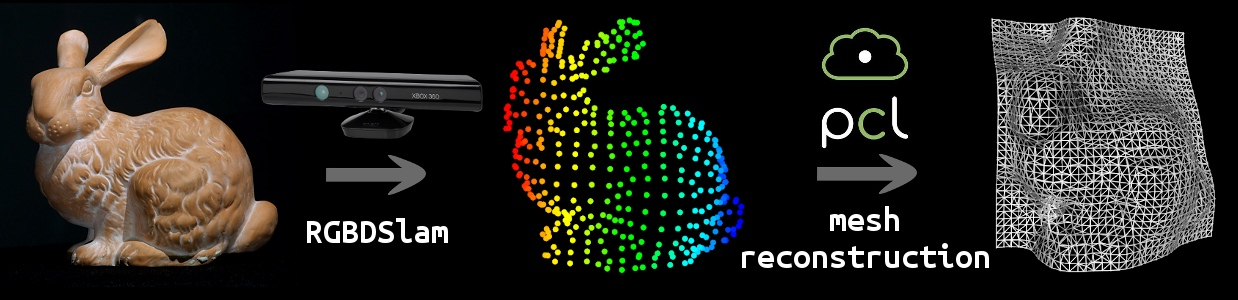
\includegraphics[scale=0.35]{figures/project-description.jpeg}
\caption[]{Grafički prikaz projekta upotrebom Standfordovog
zeca\footnotemark[1]}
\label{fig:project-description}
\end{figure}

\footnotetext[1]{%
Standford Bunny 3D model su originalno konstruirali 1994 Greg Turk i
Marc Levoy i od tada je postao najčešće upotrebljevani model za
testiranje tehnika u računalnoj grafici. \url{http://www.gvu.gatech.%
edu/people/faculty/greg.turk/bunny/bunny.html}
}

% subsection Zadatak diplomskog rada (end)
% section Uvod (end)
